\documentclass[12pt]{article}
\usepackage{MathNotes}

% Table of contents hyperlink setup, needs to be separate for some reason
\usepackage{hyperref}
\hypersetup{
 colorlinks,
 linkcolor=blue
}

\begin{document}

\title{Calculus Lecture Notes}
\author{Will Huang and Alex Zamora}
\maketitle
\tableofcontents

\newpage 

\section{Introduction}
I wrote these notes for the students of Alex Zamora's ``Calculus Club," a pilot initiative to introduce AP Calculus AB concepts to middle schoolers/rising high schoolers. The general layout of the material follows that of Strang and Herman's free online calculus textbook\footnote{Available \href{https://openstax.org/details/books/calculus-volume-1}{here}}, though adjusted slightly to suit my taste. Originally these were intended to serve as my lecture notes for sessions that I teach, but they quickly evolved into a mix of study notes, a quick reference, and an alternate textbook. 

\section{Limits}
\subsection{Introduction to Limits}
Limits form the very backbone of calculus, almost every concept and definition comes from the limit of something else. Intuitively they are quite simple: the limit of a something is simply where is appears to be going. In practice, we need a much more rigorous definition. To see why, we turn to the ancient Greeks.

In around 450 BC, Zeno, as ancient Greek philosophers tended to do, sat around thinking of paradoxes. Here are two of his most famous:
\begin{enumerate}
	\item Atalanta\footnote{Famous figure in Greek mythology} is trying to walk to the end of a path. To walk the entire path she must first walk half the path, then half the remaining path (a quarter), then half the next remaining path (an eigth), then a sixteenth, a thirty-second, etc. Since Atalanta has to walk an infinite number of paths, how can she ever finish walking the path? 
	\item Achilles\footnote{Even more famous figure in Greek mythology} is racing a tortoise\footnote{A very famous figure in fairy tale lore, famously starred in the hit movie ``Tortoise and the Hare"}. To make if fair, he gives the tortoise a head start (say 100m). Once he takes off and covers the first 100m, the tortoise would've meandered a couple more meters. Once he runs the next few meters, the tortoise will cover a few more meters, and so on so forth. So the questions is: If every time Achilles catches up to where the tortoise was prior, the tortoise remains a bit ahead, how will Achilles ever pass the tortoise?
\end{enumerate}

The astute reader may notice that these paradoxes are clearly resolvable. After all, we walk across paths all the time and obviously Achilles will eventually pass the turtle, so why are these so famous? 

The reason why these paradoxes are even talked about now is because they deal with the concept of infinity and infinitesimals (infinitely small distances). In order to have a precise mathematical way of dealing with these, we must invent new mathematics. That new mathematics is Calculus.

To introduce the idea of a limit, let's write the Atalanta (formally known as the Dichotomy) paradox in terms of limits (kind of). For Atalanta, suppose the path is 1m long and she walks at a speed of 1m/s. Then the time taken will be
\[ t = \frac{1}{2} + \frac{1}{4} + \frac{1}{8} + \frac{1}{16} + \cdots \]

Let's try to add up the terms in this sequence, if $n$ is the number of terms we add up
\begin{center}
\begin{tabular}{|c|c|c|c|c|c|c|c|c|c|}
\hline 
n & 1 & 2 & 3 & 4 & 5 & $\cdots$ & 10 & $\cdots$ & $\infty$ \\ 
\hline 
t & 1/2 & 3/4 & 7/8 & 15/16 & 31/32 & $\cdots$ & 1023/1024 & $\cdots$ & 1 \\ 
\hline 
\end{tabular} 
\end{center}

We see that as $n$ gets really, really large, then $t$ gets really close to 1. This makes sense because Atalanta should be able to walk the 1m path in 1s.

With that history lesson out of the way, let's return to the math. Take a simple function, for instance $f(x) = x$, and let's look at how it behaves around $x = 1$. There's two ways we can answer this question:
\begin{enumerate}
	\item Start from the left of the graph and see what happens as we move up to $x = 1$
	\item Start from the right of the graph and see what happens as we move down to $x = 1$
\end{enumerate}

It's pretty obvious in this case, but we see that the graph approaches $y = 1$ regardless of which direction we approach. This idea of seeing what happens when we get close to a value is formalized in the definition of a limit.

\begin{definition}[The Limit]
Let $f(x)$ be a function and $a, L$ some real numbers. If all values of $f(x)$ approach $L$ as $x$ approaches $a$, then we say that $L$ is the limit of the function $f(x)$ as $x$ approaches $a$. In symbols, we write this as
\[ \lim_{x \to a} f(x) = L \]
\end{definition}

\begin{example}
What we got from the previous simple example is that
\[ \lim_{x \to 1} x = 1 \]
\end{example}

A quick and dirty way to evaluate limits is to evaluate a bunch of values progressively closer to the value we wish to look at. If the $y$ values appears to get closer to some number, then that number is probably the limit.

\begin{example}

Consider the function $f(x) = x^2$ and suppose we want to find the limit as $x$ approaches $2$. To evaluate this limit using a table, we compute the following values:

\begin{center}
\begin{tabular}{|c|c|c|c|c|c|c|}
\hline 
x & 1.9 & 1.99 & 1.999 & 2.001 & 2.01 & 2.1 \\ 
\hline 
f(x) & 3.61 & 3.9601 & 3.996001 & 4.004001 & 4.0401 & 4.41 \\ 
\hline 
\end{tabular} 
\end{center}

From looking at this table, we can make an educated guess at the limit
\[ \lim_{x \to 2} x^2 = 4 \]

\end{example}

The method of evaluating limits using a table is very crude and, as we saw, very difficult without some form of computer assistance. Throughout mathematics, it is most common to evaluate limits algebraically. First, we discuss the notion of a one-sided limit.

\newpage 
\begin{definition}[One-Sided Limits]
Let $f(x)$ be a function and $a$ some real number. There are two different one-sided limits:
\begin{itemize}
	\item If $f(x)$ approaches a real number $L$ as $x$, where $x < a$, approaches $a$, then the \textbf{left-sided limit} of $f(x)$ as $x$ approaches $a$ is $L$, or in symbols
	\[ \lim_{x \to a^-} f(x) = L \]
	\item If $f(x)$ approaches a real number $M$ as $x$, where $x > a$, approaches $a$, then the \textbf{right-sided limit} of $f(x)$ as $x$ approaches $a$ is $M$, or in symbols
	\[ \lim_{x \to a^+} f(x) = M \]
\end{itemize}
\end{definition}

\begin{example}
Consider a piece-wise function
\[ f(x) = \begin{cases} 
x & x \leq 0 \\
x^2 + 1 & x > 0
\end{cases} \]

If we approach 0 from the left, we are on the top function. We can plug in 0 directly to find
\[ \lim_{x \to 0^-} f(x) = 0 \]

From the right we are on the bottom function. We can still plug in 0 even though the condition is $x > 0$ because limits are not about what the function actually is, rather it is about what the function is approaching. Thus
\[ \lim_{x \to 0^+} f(x) = 0^2 + 1 = 1 \]

\end{example}

This method of ``plug-and-chug" is generally how most limits will be evaluated. In the rare case that this doesn't work (for instance we end up dividing by zero), we'll need to do some more algebra.

\begin{theorem}[Two-Sided Limits]
The limit of a function $f(x)$ as $x$ approaches $a$ exists if and only if both one-sided limits exist and are equal, that is
\[ \lim_{x \to a} f(x) = \lim_{x \to a^-} f(x) = \lim_{x \to a^+} f(x) \]
\end{theorem}

Thus we cannot conclude that a limit exists unless both the left- and right-handed limits exist and are equal. 

\begin{example}
	Let $a$ and $c$ be any two real numbers, the two most basic limits are
	\[ \lim_{x \to a} c = c \qquad \lim_{x \to a} x = a \]
\end{example}


\begin{example}
	Sometimes the limit does not exist because we try to do something illegal, for instance
	\[ \lim_{x \to -4} \sqrt{x} = \varnothing \]
	because we cannot square root a negative\footnote{Technically we can, but then we would have to work in the complex plane and that requires much more complicated machinery (complex analysis)}
\end{example}

\begin{example}
	Consider a piece-wise function
	\[ f(x) = \begin{cases} 
	\sin(x) & x <= 0 \\ 
	\cos(x) & x > 0 
	\end{cases} \]
	We have the following one-sided limits
	\[ \lim_{x \to 0^-} f(x) = 0 \qquad \lim_{x \to 0^+} f(x)= 1 \]
	Since the two are not equal, the limit of $f(x)$ as $x$ approaches $0$ does not exist.
\end{example}

Sometimes we end up trying to do something illegal when we ``plug-and-chug," but that does not always mean the limit doesn't exist. In some cases infinity (or negative infinity) is a perfectly valid answer\footnote{Though it can be debated if these limits actually exist}. Identifying infinite limits requires a bit of brainpower. The process is similar to making a table of values but we don't actually do it. It's easiest to demonstrate with examples:

\begin{example}
	Consider the function $f(x) = 1/x$ as $x$ approaches 0. From the right side we get smaller and smaller $x$ values, which means that $f(x)$ gets larger and larger. Thus we can write
	\[ \lim_{x \to 0^+} f(x) = \infty \]
	From the left side we also get smaller and smaller values, but negative. Thus rather than get bigger, $f(x)$ gets more and more negative, so we write
	\[ \lim_{x \to 0^-} f(x) = -\infty \]
	Since these two one-sided limits are not the same, the limit does not exist.
\end{example}

\begin{example}
	Now consider the function $f(x) = 1/x^2$. We can use a similar argument from last time, but since the denominator is squared, the function will always be positive. Thus
	\[ \lim_{x \to 0} f(x) = \lim_{x \to 0^-} f(x) = \lim_{x \to 0^+} f(x) = \infty \]
\end{example}

The value of the limit is not the only place where infinity could exist, we may be interested in the behavior of the function as $x$ itself approach positive/negative infinity. Again, we demonstrate with an example:

\begin{example}
	Consider the function $f(x) = 1/x$ again. Suppose we want to know the limit as $x$ goes to infinity. To do this, we think about what happens as $x$ gets larger and larger. Clearly $f(x)$ would get smaller and smaller as the denominator grows, so
	\[ \lim_{x \to \infty} f(x) = 0 \]
	Similarly, we can show that
	\[ \lim_{x \to -\infty} f(x) = 0 \]
\end{example}

Limits with infinity gives us a way to find asymptotes without having to draw a graph.
\begin{theorem}
	Let $f(x)$ be a function and $a$ a real number. The line $x = a$ is a vertical asymptote if both one-sided limits are positive or negative infinity. In symbols
	\[ \lim_{x \to a^-} f(x) = \pm \infty \qquad \lim_{x \to a^+} f(x) = \pm \infty \]
	Note that this does not mean the limit itself is defined as we say in the case of $f(x) = 1/x$. 
	
	The line $y = a$ is a horizontal asymptote if the limit as $x$ goes to positive or negative infinity is $a$.
	\[ \lim_{x \to -\infty} f(x) = a \qquad \text{ or } \qquad \lim_{x \to \infty} f(x) = a \]
\end{theorem}

\begin{example}
	Let's find all asymptotes for the following function
	\[ f(x) = \frac{1}{1 - x} + 3 \]
	First we do the horizontal asymptotes
	\[ \lim_{x \to -\infty} f(x) = \lim_{x \to \infty} f(x) = 3 \]
	so $y = 3$ is a horizontal asymptote for this function.
	
	It's a bit harder to see the vertical asymptotes right away, but a good way to find them is to look for ``divide by zeros" and then evaluate the limits. In this case we consider $x = 1$
	\[ \lim_{x \to 1^-} = \infty \qquad \lim_{x \to 1^+} = - \infty \]
	Notice that the left handed limit is positive infinity this time. This is because when $x < 1$, the denominator is very small but positive. When dealing with infinities, it is very important to make sure you have the right one.
\end{example}

If we are given a graph of a function, we can evaluate limits visually by examining the behavior of the graph. For instance if we wanted to evaluate a left-handed limit, we can place our pencil a bit to the left of the point and trace the line up to that point. The height that we appear to be approaching is the limit. Remember: the limit is what the function appears to approaching, not what it actually is.\footnote{If it helps, you may think of limits as "It is not the destination that matters, but the journey"}

\begin{example} 
Consider the following graph of a function $f(x)$
\begin{center}
	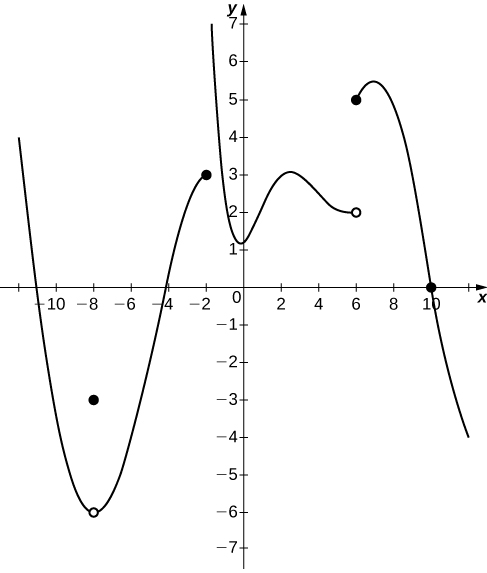
\includegraphics[scale=1]{images/Figure 2.2.1.jpg}
\end{center}

At $x = -8$, we see that from the left and the right we are approaching the same value. The fact that $f(-8) = -3$ does not matter, the limits are
\[ \lim_{x \to -8^-} f(x) = \lim_{x \to -8^+} f(x) = \lim_{x \to -8} f(x) = -6 \]

At $x = -2$ the graph has different behavior depending on if we are on the left or right. If we trace the graph coming from the left, we will approach $y = -2$ and in fact this is also the value of $f(-2)$. If we come from the right then we go straight up to $+ \infty$. Thus
\[ \lim_{x \to -2^-} f(x) = 3 \qquad \lim_{x \to -2^+} = \infty \qquad \lim_{x \to -2} = \varnothing \]

The remaining two interesting points, $x = 6$ and $x = 10$, will be left as an exercise to the sufficiently motivated and astute reader.
\end{example}

\newpage 
\subsection{Techniques for Limits}

Now that we've brute forced our way through a couple limits, it is time to find a way to use those previous results to evaluate new limits. A lot of these laws/rules may seem obvious but it is important to state them nonetheless.

\begin{theorem}[Properties of Limits]
	Let $f(x)$ and $g(x)$ be functions, $a$ a real number, and suppose $f,g$ have the following limits
	\[ \lim_{x \to a} f(x) = L \qquad \lim_{x \to a} g(x) = M \]
	
	Then we have the following properties, let $c$ be a constant
	\begin{align*}
		\lim_{x \to a} f(x) \pm g(x) &= \lim_{x \to a} f(x) \pm \lim_{x \to a} g(x) = L \pm M \\
		\lim_{x \to a} f(x)g(x) &= \lim_{x \to a} f(x) \cdot \lim_{x \to a} g(x) = L \cdot M \\
		\lim_{x \to a} cf(x) &= c \cdot \lim_{x \to a} f(x) = c \cdot L \\
		\lim_{x \to a} \frac{f(x)}{g(x)} &= \frac{\lim_{x \to a} f(x)}{\lim_{x \to a} g(x)} = \frac{L}{M} \qquad \text{ if $M \neq 0$} \\
		\lim_{x \to a} (f(x))^n &= \qty(\lim_{x \to a} f(x))^n = L^n \\
		\lim_{x \to a} \sqrt[n]{f(x)} &= \sqrt[n]{\lim_{x \to a} f(x)} = \sqrt[n]{L}
	\end{align*}
	
	The last result holds for all $x$ if $n$ is odd and all $x \geq 0$ if $n$ is even (these also happen to be the domains of $\sqrt[n]{x}$ for odd/even $n$).
\end{theorem}

These laws give the ``plug and chug" strategy a more mathematical reasoning. Since we know the two basic limits
\[ \lim_{x \to a} c = c \qquad \lim_{x \to a} x = a \]
we can use the limit laws to manipulate them into the function we are interested in. 

\begin{example}
	Consider the function
	\[ f(x) = \frac{x^2 + 3x - 10}{x^3 - 2x} \]
	
	The using the basic limits, we can evaluate the limit
	\[ \lim_{x \to 2} f(x) = \frac{2^2 + 3 \cdot 2 - 10}{2^3 - 2 \cdot 2} = \frac{0}{4} = 0 \]
\end{example}

It is worth noting that these laws all apply the one-sided limits as well.

There are many tricks to evaluating limits, we'll cover a few of the most common ones in the ensuing exercises.
\begin{example}
	Consider the function
	\[ f(x) = \frac{x^2 + 2x - 3}{x^2 - 1} \]
	
	If we tried to evaluate the limit as $x$ approaches 1, then we would end up dividing by zero. To avoid this we must first factor the top and bottom
	\[ f(x) = \frac{(x + 3)(x - 1)}{(x + 1)(x - 1)} = \frac{x + 3}{x + 1} \]
	Now we see that since a term cancels, we can use the limit laws to evaluate
	\[ \lim_{x \to 1} f(x) = \frac{1 + 3}{1 + 1} = 2 \]
\end{example}

\begin{example}
	When working with square roots it is common to get a function of the form
	\[ f(x) = \frac{\sqrt{x + 1} - 1}{x} \]
	
	If we tried to evaluate the limit as $x$ approaches 0 it would appear to seem that we are stuck. Furthermore there is nothing to factor, so what is there left to do? It turns out that we can use the fact that $x^2 - a^2 = (x + a)(x - a)$ change the fraction. This is known as multiplying by the conjugate, lets see it in action:
	\begin{align*}
		f(x) &= \frac{\sqrt{x + 1} - 1}{x} \cdot \qty(\frac{\sqrt{x + 1} + 1}{\sqrt{x + 1} + 1}) = \frac{(\sqrt{x + 1})^2 - 1^2}{x(\sqrt{x + 1} + 1)} \\
		&= \frac{x + 1 - 1}{x(\sqrt{x + 1} + 1)} = \frac{x}{x(\sqrt{x + 1} + 1)}\\
		&= \frac{1}{\sqrt{x + 1} + 1}
	\end{align*}
	
	This sort of algebraic manipulation is allowed because at the end of the day, all we did was multiply by 1. With the function in this form, we can now evaluate the limit
	\[ \lim_{x \to 0} f(x) = \frac{1}{\sqrt{0 + 1} + 1} = \frac{1}{2} \]
\end{example}

\begin{example}
	When evaluating limits, one should always try to simplify the function as much as possible before preceding. Consider the function
	\[ f(x) = \frac{1}{x} - \frac{3}{x(x + 3)} \]
	
	If we tried to evaluate the limit as $x$ goes to 0, we may be tempted to either say it does not exist or is an asymptote due to the $1/x$. But if we took the time to simply, we find
	\[ f(x) = \frac{x + 3}{x(x + 3)} - \frac{3}{x(x + 3)} = \frac{x}{x(x + 3)} = \frac{1}{x + 3} \]
	Now we can evaluate
	\[ \lim_{x \to 0} f(x) = \frac{1}{0 + 3} = \frac{1}{3} \]
\end{example}

For more complicated limits we may sometimes use the squeeze (or sandwich) theorem when applicable.
\begin{theorem}[Squeeze Theorem]
	Let $f(x), g(x), h(x)$ be functions defined for all $x \neq a$ in an open interval containing $a$. If
	\[ f(x) \leq g(x) \leq h(x) \]
	The their limits obey
	\[ \lim_{x \to a} f(x) \leq \lim_{x \to a} g(x) \leq \lim_{x \to a} h(x) \]
	
	In particular if
	\[ \lim_{x \to a} f(x) = \lim_{x \to a} h(x) = L \]
	then it must be the case that
	\[ \lim_{x \to a} g(x) = L \]
\end{theorem}

To see how we may use this theorem to solve otherwise impossible limits, consider the following example.

\begin{example}
	Suppose we have a function
	\[ f(x) = x \cos(\frac{1}{x}) \]
	and we wish to evaluate the limit as $x$ goes to 0. We can't use the limit laws because then we'd be dividing by zero, so instead we note that
	\[ -1 \leq \cos(x) \leq 1 \qquad \text{ and so } \qquad -x \leq f(x) \leq x \]
	
	It doesn't matter what's inside the cosine because it will always be between -1 and +1. Thus we just need to compute
	\[ \lim_{x \to 0} -x = 0 \qquad \lim_{x \to 0} x = 0 \]
	and we are able to conclude, using the squeeze theorem,
	\[ \lim_{x \to 0} f(x) = 0 \]
\end{example}

Note that in order to actually get a limit out of the squeeze theorem, the limit on both sides of the inequality must be the same. If they are different, then the squeeze limit does not tell us anything.

\begin{Optional}[Important Trigonometric Limits]
For this subsection I will use without proof the following limits\footnote{A geometric proof of the first limit using the squeeze theorem is provided in the textbook and the second can be found by multiplying by the conjugate}
\[ \lim_{x \to 0} \frac{\sin(x)}{x} = 1 \qquad \lim_{x \to 0} \frac{1 - \cos x}{x} = 0\]

Let's see how we can use these two limits to evaluate a deceptively difficult limit

\begin{example}
	Consider the function
	\[ f(x) = \frac{\sin^2(3x)}{\sin(2x)} \]
	
	We want to evaluate the limit as $x$ approaches $0$. At first glance, we don't really see much that we can do. After all, both the numerator and denominator goes to zero. However, before we give up and quit math forever, we notice that there is one (indeed the only) thing to do: rewrite the numerator. 
	\[ f(x) = \frac{1 - \cos^2(3x)}{\sin(2x)} = \frac{(1 + \cos(3x))(1 - \cos(3x))}{\sin(2x)} \]
	
	We now remember that we've seen part of this numerator before, it's the same numerator in the limit we first introduced! But we're missing the denominator, furthermore the function instead the cosine is $x$, not $3x$. To fix this, we turn to the old trick: multiply by 1. This also fixes the sine in the denominator
	\begin{align*}
		f(x) &= \frac{(1 + \cos(3x))(1 - \cos(3x))}{\sin(2x)} \cdot \qty(\frac{2x}{2x}) \cdot \qty(\frac{3x}{3x}) \\
		&= \qty(\frac{2x}{\sin(2x)}) \cdot \qty(\frac{1 - \cos(3x)}{3x}) \cdot \qty(\frac{2x(1 + \cos(3x))}{3x}) \\
		&= \frac{2}{3} \qty(\frac{1}{\sin(2x)/2x}) \qty(\frac{1 - \cos(3x)}{3x}) (1 + \cos(3x))
	\end{align*}
	Now we can evaluate the limit
	\[ \lim_{x \to 0} f(x) = \frac{2}{3} \cdot \frac{1}{1} \cdot 0 \cdot (1 + 0) = 0 \]
\end{example}

\end{Optional}

\newpage 
\subsection{Continuity}

% Definition of continuity
% Types of discontinuity
% Interval continuity + examples
% Limit composition
% Intermediate value theorem

\newpage 
\subsection{Hard Topic: Precise Definition of a Limit}

% Introduction to epsilon delta
% Examples
% Proving a limit law
% Very hard example/proof
\section{Derivatives}
\subsection{Introduction to Derivatives}

There are three ideas at the core of calculus. We've already covered one so far, the limit, and you've all (mostly) survived so now we can move on to the derivative. Here's the problem: slopes of lines is easy, take any two points and use the slope formula. But if I point to some point on a quadratic and ask you to give me the slope then you're shit out of luck. Luckily with the power of god and \st{anime} limits on your side, we can rectify this issue (in just a few more pages too!).

To begin, what exactly does the slope at a single point mean. We can easily find the slope between two points by drawing a line between them, but for a curve there's no lines. For the case of a curve, the slope at a single point will be the slope of line which \emph{just barely} touches the curve at that point. In other words we want the slope of the tangent line of the curve at that point. But to find the slope of a tangent line, we must first discuss secant lines.

As opposed to tangent lines, we get a secant line by taking two points on a curve and drawing a line through them. For instance if we have the function $f(x) = x^2$ and we want the secant line through $x = 1$ and $x = 3$, then the slope is
\[ m = \frac{f(3) - f(1)}{3 - 1} = \frac{9 - 1}{2} = 4 \]
We can make this equation much more general:

\begin{definition}[Difference Quotient]
	Let $f$ be a function which is defined (i.e. exists) on some interval. Let $x$ be some point inside that interval and $h \neq 0$ a number such that $x + h$ is still in the interval. Then the difference quotient is
	\[ Q = \frac{f(x + h) - f(x)}{h} \]
\end{definition}

A geometrical interpretation of this equation is that it is the slope of the secant line through $x$ and the point $h$ away. If we want to get the slope of the tangent line, then we simply move that second point closer and closer to the first point. In other words, we take the limit as $h$ (the horizontal distance between the two points of the secant line) goes to 0.

In the figure below, we see graphically how we can get to a tangent line by first taking a secant line and then decreasing the distance between the two points until they converge to just one. This will give a visualization for the actual definition of a derivative which represents this idea using a limit.

\begin{center}
	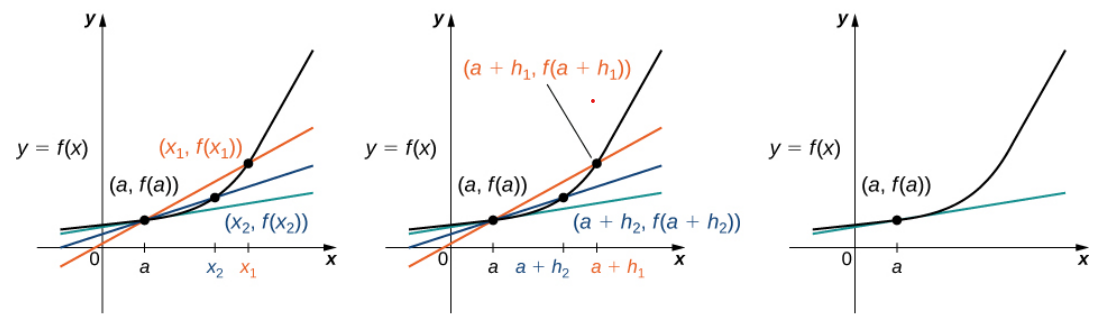
\includegraphics[scale=0.55]{images/Figure 3.1.1.png}
\end{center}

\begin{definition}[Derivatives]
	Let $f$ be a function which is defined on some open interval and $a$ some number in that interval (open interval means that $a$ cannot be either endpoint). Then the derivative of $f$ at $a$, or the slope of the tangent line at $x = a$, is given by the limit
	\[ f'(a) = \lim_{h \to 0} \frac{f(a + h) - f(a)}{h} \] 
\end{definition}

\begin{example}
	Let's take perhaps the simplest example (asides from constants) known to man, a linear function
	\[ f(x) = x \]
	Then the derivative, the slope of the tangent line, at any point $x = a$ is
	\[ f'(a) = \lim_{h \to 0} \frac{(a + h) - a}{h} = \lim_{h \to 0} \frac{h}{h} = \lim_{h \to 0} 1 = 1 \]
	This makes sense because the tangent line to a line is the line itself and the slope of a line does not change.
\end{example}

\begin{example}
	Here's a more complicated example
	\[ f(x) = x^2 \]
	Again we'll be general and consider any point $x = a$.
	\begin{align*}
		f'(a) &= \lim_{h \to 0} \frac{(a + h)^2 - a^2}{h} = \lim_{h \to 0} \frac{a^2 + 2ah + h^2 - a^2}{h} \\
		&= \lim_{h \to 0} \frac{2ah + h^2}{h} = \lim_{h \to 0} 2a + h \\
		&= 2a
	\end{align*}
	So the slope of a tangent line at some $x$ value is two times that $x$ value.
\end{example}

\newpage 
\begin{example}
	One more example
	\[ f(x) = \sqrt{x} \]
	This limit is slightly more involved
	\begin{align*}
		f'(a) &= \lim_{h \to 0} \frac{\sqrt{a + h} - \sqrt{a}}{h} \\
		&= \lim_{h \to 0} \frac{a + h - a}{h (\sqrt{a + h} + \sqrt{a})} = \lim_{h \to 0} \frac{h}{h(\sqrt{a + h} + \sqrt{a})} \\
		&= \lim_{h \to 0} \frac{1}{\sqrt{a + h} + \sqrt{a}} = \frac{1}{\sqrt{a} + \sqrt{a}} \\
		&= \frac{1}{2 \sqrt{a}}
	\end{align*}
\end{example}

Sometimes you might hear a derivative referred to as an \emph{instantaneous rate of change}, this comes from physics where the slope of something represents its rate of change. With this in mind, let's do a couple more examples but set in the real world.

\begin{example}
	Suppose we chuck a ball into the air such that its height is given by
	\[ y(t) = -5t^2 + 10t \]
	We want to know exactly how fast the ball is falling when it hits the ground, so first we solve for the time when it does hit the ground.
	\[ y(t) = -5t(t - 2) = 0 \thus t = 0, 2 \]
	$t = 0$ is when we first yeet the ball, so $t = 2$ is when it comes back down. Now we can do the limit
	\begin{align*}
		v(2) = y'(2) &= \lim_{h \to 0} \frac{y(t + h) - y(t)}{h} \\
		&= \lim_{h \to 0} \frac{(-5(2 + h)^2 + 10(2 + h)) - (-5(2)^2 + 10(2))}{h} \\
		&= \lim_{h \to 0} \frac{-5(4 + 4h + h^2) + 20 + 10h - 0}{h} \\
		&= \lim_{h \to 0} \frac{-10h - 5h^2}{h} = \lim_{h \to 0} -10 - 5h \\
		&= -10
	\end{align*}
	For that have done some physics before may notice that I set up this problem such that we throw the ball up in the air with speed $\SI{10}{m/s}$ (and rounded the acceleration due to gravity to $\SI{10}{m/s^2}$). The fact that the ball hits the ground exactly as fast as we threw it up is a neat result and you can verify that this is the case for other initial velocities as well.
\end{example}

So far we've been evaluating the derivative at a specific point, but there is nothing really stopping us from defining a function which gives derivatives for an arbitrary input. This function, read ``f prime," is what we will refer to as the derivative from here on out.
\[ f'(x) = \lim_{h \to 0} \frac{f(x + h) - f(x)}{h} \]

We will investigate exactly what the derivative means more later, but we can still gain a basic understanding right now. The derivative is a function which returns the slope of a tangent line at any point $x$. In a certain way, this is the ``slope" at that point, how fast the function is going up or down. So for now, we can think of the derivative as a function which tells use how fast a function is increase (or decreasing if $f'(x) < 0$). 

There is a crucial connection between derivative and continuity.
\begin{theorem}[Continuity and Differentiability]
	If a function $f(x)$ is differentiable (i.e. the derivative exists) at $x = a$, then it must be continuous at $x = a$.
\end{theorem}

This gives us a shortcut from the limits we introduced last chapter. If we can somehow compute a derivative (function) and that function is not undefined at some point, then we will know that function is also continuous there. Now the curious reader may ask "Well what about the other way around? Are continuous functions always differentiable? " The answer is no. 

\begin{center}
	
\includegraphics[scale=1]{images/Figure 3.1.2.png} 
\end{center}

Once we take the derivative of a function, there is nothing stopping us from doing it again. For instance, using derivatives we found in previous examples we can take a double derivative (and more, which I will leave for you to verify)
\[ f(x) = x^2 \thus 2x \thus 2 \thus 0 \]

These are called ``higher-order" derivatives, but generally we will refer to them by the amount of derivatives taken. Going back to the example of $f(x) = x^2$; the first derivative is $2x$, the second derivative is $2$ and the third derivative is $0$. This pattern continues, for any function $f$, the $n$-th derivative will be the function resulting from taking the derivative $n$ times.

There is two (three if you're a physicist and four if you're a mathematician) ways to write a derivative. Suppose we have a function $f(x)$, then Lagrange notation\footnote{You do not need to know what this is called.} denotes the derivatives as
\[ f'(x) \qquad f''(x) \qquad f'''(x) \qquad f^{(4)}(x) \qquad \cdots \qquad f^{(n)}(x)\]
It is customary to use the dashes for the first three derivatives, but start writing the numbers for higher derivatives. The other common notation in calculus is Liebniz's notation
\[ \dv{f}{x} \qquad \dv[2]{f}{x} \qquad \dv[3]{f}{x} \qquad \dv[4]{f}{x} \qquad \cdots \qquad \dv[n]{f}{x} \]
The reason for the numbers being where they are comes from the following
\[ \dv{x} \qty( \dv{x} \qty( \dv{f}{x} )) = \dv{x} \qty( \dv[2]{f}{x} ) = \dv[3]{f}{x} \]
Though don't write $\dd^3x^3$ on the bottom, to make sense of this you should think of the entire $\dd x$ as its own block (add invisible parentheses if that makes you feel better).

Having to go through an entire limit to get a derivative is a bit tedious, especially as the functions we consider become more and more complicated. Just like how we can build arbitrary limits out of basic ones, there are rules that let us construct more advanced derivatives from basic ones. 

\begin{example}
	First we need to establish two basic results, one we did earlier and the other can be easily proven
	\[ \dv{x}(c) = 0 \qquad \dv{x}(x) = 1 \] 
\end{example}

\newpage 
Now we introduce perhaps the most useful derivative rule in calculus:

\begin{theorem}[The Power Rule]
	For any real number $n \neq 0$, the derivative of the function $f(x) = x^n$ is 
	\[ f'(x) = n x^{n - 1} \]
\end{theorem}

It is important to note that this holds for any nonzero exponent, negative numbers and fractions included.

\begin{example}
	Let's rapid fire run through a bunch of examples, some of which we did using the limit definition earlier and others you will have to take my word that the limit definition gives the same result.
	\[ \dv{x}(x^2) = 2x \qquad \dv{x}(x^3) = 3x^2 \qquad \dv{x}(\sqrt{x}) = \frac{1}{2}x^{-1/2} = \frac{1}{2\sqrt{x}} \]
	\[ \dv{x}(\frac{1}{x}) = \dv{x}(x^{-1}) = x^{-2} = \frac{1}{x^2} \qquad \dv{x}(x^{3/4}) = \frac{3}{4}x^{-1/4} = \frac{3}{4\sqrt[4]{x}} \]
\end{example}

Another simple but useful rule is the constant rule, essentially stating that you can pull out constant coefficients when computing a derivative.
\[ \dv{x}(cf(x)) = c \dv{x}(f(x)) = c f'(x) \]

The final piece of the puzzle is the sum rule, using this we can start taking derivatives of basically every polynomial function.

\begin{theorem}[Sum Rule]
	Let $f(x)$ and $g(x)$ be two differentiable functions, then
	\[ \dv{x}(f(x) + g(x)) = \dv{f}{x} + \dv{g}{x} = f'(x) + g'(x) \]
\end{theorem}

To see this in action, we will run through the derivative of a simple polynomial while elaborating every single step we take. In general we won't have to be this verbose, but it is helpful to do so at least once to see how these rules are used.

\begin{example}
	Consider the function $f(x) = 3x^2 + 2x + 4$, the derivative is
	\begin{align*}
		f'(x) &= (3x^2 + 2x + 4)' \\
		&= (3x^2)' + (2x)' + (4)' \\
		&= 3 (x^2)' + 2 (x)' + 4(1)' \\
		&= 3(2x) + 2(1) + 4(0) \\
		&= 6x + 2
	\end{align*}
\end{example}

The sum rule in conjunction with the constant rule means that we can take derivative of subtracted functions as well. The last two operations to complete our collection are multiplication and division.

\begin{theorem}[Product Rule]
	Let $f(x)$ and $g(x)$ be differentiable functions, then
	\[ \dv{x}(f(x)g(x)) = f'(x)g(x) + f(x)g'(x) \]
\end{theorem}

The becomes useful when we have factored polynomials.

\begin{example}
	Take the derivative of $f(x) = (x^2 + 3)(x^2 - 4x)$. One way is to expand
	\[ f(x) = x^4 -4x^3 + 3x^2 - 12x \thus f'(x) = 4x^3 - 12x + 6x - 12 \]
	This is not feasible when the factors get longer, instead we can use the product rule
	\[ f'(x) = (x^2 +3)'(x^2 - 4x) + (x^2 + 3)(x^2 - 4x)' = (2x)(x^2 - 4x) + (2x)(x^2 - 4x) \]
\end{example}

You may complain ``wait, we haven't expanded the final result, this doesn't actually stop any algebra from happening." However this answer is just as good because often we are concerned with a single point. Regardless of the form it's in, we can still plug in values to get derivatives at specific points.

\begin{theorem}[Quotient Rule]
	Let $f(x)$ and $g(x)$ be differentiable functions, then
	\[ \dv{x}(\frac{f(x)}{g(x)}) = \frac{f'(x)g(x) - f(x)g'(x)}{(g(x))^2} \]
\end{theorem}

If this seems a bit hard to remember, the standard trick is to repeat to yourself "low d high minus high d low over low squared" which means to take the bottom function times the derivative of the top function and then subtract the top function times the derivative of the bottom function, all divided by the bottom squared. Another way is to just write the product rule on top but with a minus sign.

\begin{example}
	For a simple example, consider the function
	\[ f(x) = \frac{x + 1}{x - 1} \]
	One way is to use product rule, but then we would have to derive $1/(x+1)$ which we cannot do with normal rules, so instead we have to use quotient rule.
	\[ f'(x) = \frac{(x + 1)'(x - 1) - (x + 1)(x - 1)'}{(x - 1)^2} = \frac{(x - 1) - (x + 1)}{(x - 1)^2} = -\frac{2}{(x - 1)^2}\]
\end{example}

Let's put everything we've learned together with a more complicated example

\begin{example}
	Consider the function
	\[ f(x) = \frac{(2x + 1)(3x^2 + 4x + 2)}{x^2 - 1} \]
	The derivative is (we'll skip some algebra because you are seasoned derivers now)
	\begin{align*}
		f'(x) &= \frac{(2(3x^2 + 4x + 2) + (2x + 1)(6x + 4))(x^2 - 1) - (2x + 1)(3x^2 + 4x + 2)(2x)}{(x^2 - 1)^2} \\
		&= \frac{(18x^2 + 22x + 8)(x^2 - 1) - (4x^2 + 2x)(3x^2 + 4x + 2)}{(x^2 - 1)^2} \\
		&= \frac{6x^4 - 26x^2 - 26x - 8}{(x^2 - 1)^2}
	\end{align*}
\end{example}

\newpage 
\subsection{Applications of Derivatives}
Just like how we can find limits visually from a graph, we can also guess how the derivative of a function looks like by investigating its graph. There isn't a concrete procedure, but the general idea is:
\begin{itemize}
	\item If the function is going up, the derivative is positive. Vice versa for going down
	\item A horizontal tangent means the derivative is zero
	\item If the rate at which is function is growing is also growing, then the derivative should slope upwards. Similar logic applies to the other four cases.
\end{itemize}

\begin{example}
	The function $f(x)$ and $f'(x)$ are shown below
	\begin{center}
		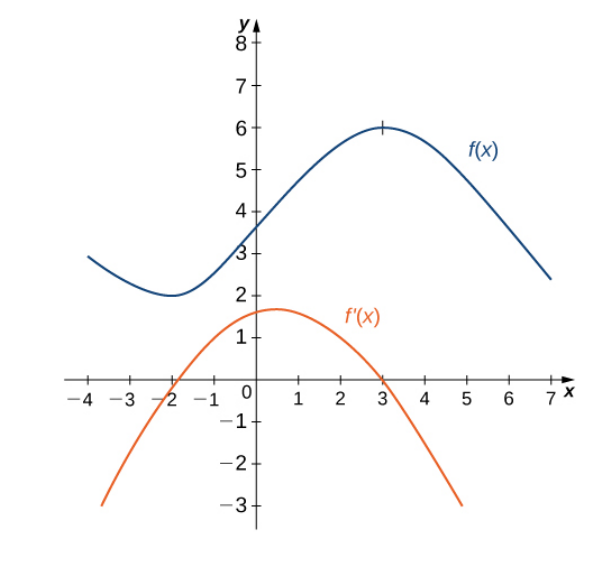
\includegraphics[scale=0.75]{images/Figure 3.2.1.png} 
	\end{center}
\end{example}

\begin{example}
	For the function $f(x) = x^2 - 3x$, where is there a horizontal derivative?
	
	To answer this question we set the derivative to zero
	\[ f'(x) = 2x - 3 = 0 \thus x = \frac{3}{2} \]
	In particular the point $(3/2, 9/4)$ is a horizontal tangent. Observant readers may notice that this is the vertex of the parabola. In fact, the vertex of a quadratic will always have zero derivative.
\end{example}

We know that the average rate of a change of a function is the quotient
\[ \frac{f(a + h) - f(a)}{h} \]
For small values of $h$, we can pretend the function is just a line and estimate
\[ f'(a) \approx \frac{f(a + h) - f(a)}{h} \thus f(a + h) \approx f(a) + h f'(a) \]
This technique, known as linear approximation, lets us estimate the function using a known value and its derivative. 

\begin{example}
	Suppose we have a function $f(x)$ such that
	\[ f(5) = 10 \qquad f'(5) = 2 \]
	We can estimate the function at 6 using a linear approximation
	\[ f(7) \approx f(5) + 2f'(5) = 14 \]
\end{example}

If this seems a bit abstract, here's something more concrete.

\begin{example}
	We can use this approximation to estimate square roots. We know that 
	\[ f(x) = \sqrt{x} \thus f'(x) = \frac{1}{2\sqrt{x}} \]
	We also know that $\sqrt{4} = 2$, so we can estimate
	\begin{align*}
		\sqrt{5} &\approx 2 + \frac{1}{2\sqrt{4}} =  2.25 \text{ vs } 2.24\\
		\sqrt{6} &\approx 2 + 2 \cdot \frac{1}{2\sqrt{4}} =  2.5 \text{ vs } 2.45 \\
		\sqrt{7} &\approx 2 + 3 \cdot \frac{1}{2\sqrt{4}} =  2.75 \text{ vs } 2.65 \\
		\sqrt{8} &\approx 2 + 4 \cdot \frac{1}{2\sqrt{4}} =  3 \\
	\end{align*}
	Note that the approximate gets worse the further we are away from our reference point. 
\end{example}

A linear approximation is an example of a first order Taylor series, we can use the higher order derivatives to refine our approximation in a (much) later chapter.

Newton invented Calculus to provide a rigorous mathematical backing for his laws of motion. We will explore a bit of that here. 

\begin{definition}[Equations of Motion]
	Suppose the motion (position) of a particle over time is given by the function $x(t)$. Then the velocity of that particle is
	\[ v(t) = x'(t) \]
	The absolute value of velocity (i.e. its magnitude) is the particle's speed. The derivative of velocity gives its acceleration
	\[ a(t) = v'(t) = x''(t) \]
	The derivative of acceleration, the third derivative of position, is its jerk
	\[ j(t) = a'(t) = x''(t) = x'''(t) \]
	The next few higher order derivatives of position are snap, crack, and pop. You do not need to know the derivatives of position past acceleration.
\end{definition}

\begin{example}
	Consider a particle which moves according to
	\[ x(t) = t^3 - t^2 + 25 \]
	It's velocity and acceleration at a particular time is 
	\[ v(t) = 3t^2 - 2t \qquad a(t) = 6t - 2 \]
	From this we see that it is speeding up for $t > 1/3$ and slowing down otherwise. We can also solve
	\[ v(t) = t(3t - 2) > 0 \thus t < 0, t > 2/3 \]
	So for $t > 2/3$, the particle is moving forward.
\end{example}

In biology, particularly ecology, derivatives play a key role in modeling population dynamics. For instance, if the population of a city triples every 5 years and there are 10,000 people in the current year. Then
\[ P'(0) \approx \frac{P(5) - P(0)}{5 - 0} = \frac{30000 - 10000}{5} = 4000 \]
If we want to estimate the population in 3 years, then
\[ P(3) \approx P(0) + 3P'(0) = 10000 + 3 \cdot 4000 = 22000 \]

Population dynamics is more accurately modeled using the exponential function and differential equations, we will return to this example later when you learn what these are.

Derivatives are also used in economics when discuss the behavior of firms or other agents. In certain instances, we can use them to give optimal answers to questions like "How much should I produce of a certain good?" or "How much should I charge for this service?" 

\begin{example}
	In a monopolistically competitive market, the demand curve faced by a firm is equal to population demand due to market power. If the firm wishes to sell $x$ quantity of some good, then the price is given by
	\[ p(x) = 100 - x \]
	In other words, the firm can charge $50$ and sell 50 units or charge $99$ and only sell 1. The revenue is simply price times quantity and the derivative gives what is known as the marginal revenue: the additional revenue gained from selling one more unit.
	\[ R(x) = x p(x) = 100 x - x^2 \thus MR(x) = R'(x) = 100 - 2x \]
	Revenue is maximized when $MR = 0$ (you will learn why later), which occurs at exactly 50 goods sold. However this does not actually maximize profits.
	
	The cost to produce $x$ units of a good will be impacted by economies of scale. Just like revenue, we can differentiate to get the marginal cost: the cost to produce one more unit
	\[ C(x) = 16 + x^2 \thus MC(x) = C'(x) = 2x \]
	Profit in a monopolistic market is achieved when marginal cost equals marginal revenue
	\[ 100 - 2x = 2x \thus x = 25 \]
	and we see that the optimal quantity in this market is 25 units.
\end{example}

\newpage
\subsection{The Chain Rule}

\newpage 
\subsection{Derivatives of Special Functions}
In this section we give the derivatives of functions not covered by the power rule, for instance trigonometric functions and exponential functions. We will start with the trig functions.

We compute the derivative of sine directly from the limit definition using sum to product identities
\begin{align*}
	\dv{x} (\sin x) &= \lim_{h \to 0} \frac{\sin(x + h) - \sin(x)}{h} \\
	&= \lim_{h \to 0} \frac{2\sin(h/2)\cos(x + h/2)}{h} \\
	&= \lim_{h \to 0} \frac{\sin(h/2)}{h/2} \cdot \lim_{h \to 0} \cos(x + h/2) \\
	&= 1 \cdot \lim_{h \to 0} \cos(x + h/2) \\
	&= \cos(x) \\
	\dv{x} (\cos x) &= \lim_{h \to 0} \frac{\cos(x + h) - \cos(x)}{h} \\
	&= \lim_{h \to 0} \frac{-2\sin(h/2)\sin(x + h/2)}{h} \\
	&= \lim_{h \to 0} \frac{\sin(h/2)}{h/2} \cdot \lim_{h \to 0} -\sin(x + h/2) \\
	&= 1 \cdot \lim_{h \to 0} -\sin(x + h/2) \\
	&= -\sin(x) 
\end{align*}

The derivative of tangent comes from quotient rule
\begin{align*}
	\dv{x} (\tan x) &= \dv{x} \qty(\frac{\sin x}{\cos x}) \\
	&= \frac{(\cos x)(\cos x) - (\sin x)(-\sin x)}{\cos^2 x} \\
	&= \frac{\cos^2 x + \sin^2 x}{\cos^2 x} \\
	&= \frac{1}{\cos^2 x} = \sec^2 x 
\end{align*}

Now that we can take derivatives of trig functions, we have a more useful use case of the product rule.
\begin{example}
	Consider the function
	\[ f(x) = x^2 \sin x \]
	This product cannot simply be expanded, we are forced to use product rule
	\[ f'(x) = 2x \sin x + x^2 \cos x \]
\end{example}

Using quotient rule, we can take derivatives of the remaining trig functions. I'll list them here for your convenience:
\begin{proposition}[Trig Derivatives]
	\begin{align*}
		\dv{x} (\sin x) &= \cos x \\
		\dv{x} (\cos x) &= -\sin x \\
		\dv{x} (\tan x) &= \frac{1}{\cos^2 x} = \sec^2 x \\
		\dv{x} (\csc x) &= - \frac{\cos x}{\sin^2 x} = -\csc x \cot x \\
		\dv{x} (\sec x) &= \frac{\sin x}{\cos^2 x} = \sec x \tan x \\
		\dv{x} (\cot x) &= -\frac{1}{\sin^2 x} = -\csc^2 x \\
	\end{align*}
\end{proposition}

Note that because sine and cosine are related by derivatives, we have the chain
\[ \sin x \thus \cos x \thus -\sin x \thus -\cos x \thus \sin x \thus \cdots \]
This is our first example of a function which is both infinitely differentiable and has nontrivial higher order derivatives. Compare this to polynomials, which always end up going to 0 if you take enough derivatives.

\begin{example}
	Suppose we want to know the equation of the tangent line of the function
	\[ f(x) = \sin x \cos x \]
	at the point $x = \pi$. First note that the derivative is
	\[ f'(x) = (\cos x)(\cos x) + (\sin x)(-\sin x) = \cos^2 x - \sin^2 x = \cos(2x) \]
	Recall that the derivative gives us the slope of the tangent line, it is $f'(\pi) = 1$. Now all we need is a point. The tangent line touches the function at only one point, that point must be the value of the function at $x = \pi$, which is $f(\pi) = 0$. The easiest way to find the equation is to use point slope form and convert if necessary
	\[ y - 0 = 1 \cdot (x - \pi) \thus y = x - \pi \]
\end{example}

\begin{example}
	A particle undergoing simple harmonic motion (for instance a mass on an ideal spring) has equation
	\[ x(t) = 5 \cos(t) \]
	We can use this to find the velocity at any time $t$
	\[ v(t) = x'(t) = -5 \sin(t) \]
	The velocity function is also periodic, by looking more closely we see that 
	\[ v(t) = 0 \iff t = 0, \pi, 2\pi, 3\pi, \cdots \]
	This is also when the spring is furthest away from the center (at $\pm 5$). The mass actually has zero speed when it reaches it's furthest point and this happens infinitely many times.
\end{example}

\newpage 
\subsection{It's About the \emph{Implication}}
\subsection{Hard Topic: Derivatives for the Morbidly Curious}

\end{document}